\documentclass{webofc}

\usepackage{graphicx}
\usepackage{tabularx}
%\usepackage{cite}
\usepackage{subcaption}
\captionsetup[figure]{labelsep=period,labelfont=bf}
\captionsetup[table]{labelsep=period,labelfont=bf}

% Set serif font to Paratype
%\usepackage{paratype}
\usepackage[varg]{txfonts}
\usepackage[T1]{fontenc}

% Colours

\usepackage{xcolor}      % Colours
\usepackage{colortbl}    % Colour tables

% CERN blue is Pantone 286 = RGB 56 97 170, defined as cern@blue below
\definecolor{cern@ltblue}{rgb}{0.415686,0.611765,0.964706} % RGB 106 156 246
\definecolor{cern@blue}  {rgb}{0.219608,0.380392,0.666667} % RGB  56  97 170
\definecolor{cern@dkblue}{rgb}{0.082353,0.184314,0.364706} % RGB  21  47  93

% Complimentary colours
\definecolor{cern@ltcomp}{rgb}{0.666667,0.525490,0.219608} % RGB 170 134  56
\definecolor{cern@dkcomp}{rgb}{0.364706,0.266667,0.047059} % RGB  93  68  12

% Hyperlinks
\usepackage{hyperref}
\hypersetup{
  colorlinks=true,
  citecolor=cern@blue,
  linkcolor=cern@dkblue,
  urlcolor=cern@ltblue,
  unicode=true
}

\begin{document}
\title{\raggedright CERN Tape Archive --- from development to production \mbox{deployment}}
\author{Michael C. Davis
   \and Vlad\'imir Bahyl
   \and Germ\'an Cancio
   \and Eric Cano
   \and Julien Leduc
   \and Steven Murray\inst{1}\fnsep\thanks{\email{{michael.davis, vladimir.bahyl, german.cancio.melia, eric.cano, julien.leduc, steven.murray}@cern.ch}}}
\institute{CERN---European Organization for Nuclear Research, 1211 Geneva 23, Switzerland}

\abstract{The first production version of the CERN Tape Archive (CTA) software is planned to be released during 2019.
CTA is designed to replace CASTOR as the CERN tape archive solution, to face the scalability and performance challenges
arriving with LHC Run--3.

\hspace{1.5em}In this paper, we describe the main commonalities and differences between CTA and CASTOR. We outline the
functional enhancements and integration steps required to add the CTA tape back-end to an EOS disk
storage system. We present and discuss the different deployment and migration scenarios for replacing
the five CASTOR instances at CERN, including a description of how the File Transfer Service (FTS)
will interface with EOS and CTA.}

\maketitle

\section{Introduction}
\label{introduction}

The High Energy Physics experiments at CERN generate a deluge of data which must be efficiently archived
for later retrieval and analysis. The CERN Tape Archive (CTA) is the new tape storage system for the custodial
copy of the physics data.

CTA is a replacement for and evolution from its predecessor, CASTOR~\cite{castor2007}. While CASTOR provides tape
storage, a disk cache and staging functionality, CTA has a more simple design philosophy.
CTA is implemented as the tape back-end to the EOS disk system~\cite{eos_chep2015}, and all disk cache functions
are delegated to EOS. As EOS is already the \textit{de facto} storage system for physics analysis at CERN,
CTA aims to provide the ``best of both worlds''---EOS disk and CASTOR tape.

The main goal of CTA is to make more efficient use of the tape drives, to handle the higher data rates
anticipated during Run--3 and Run--4 of the Large Hadron Collider (LHC). In our previous paper~\cite{cta_chep2016},
we described how this was to be achieved, by introducing a pre-emptive drive scheduler which can keep tape drives
running at full speed all of the time.

\subsection{Changing Use Cases for Archival Storage}

CERN is facing two main challenges for archival storage over the next decade. First, the rate of data taking
and the total volume of data will increase exponentially due to improvements in the luminosity and availability of the
LHC and upgrades to the detectors and data acquisition system. Second, constraints in available computing
power and disk capacity will change the way in which archival storage is used by the experiments.

By mid-2018, the total integrated luminosity delivered by the LHC during Run--2 exceeded 150 fb$^{-1}$, more
than double the design luminosity~\cite{atlas_status_lishep2018}. Run--3 is expected to be similar.
After the HL-LHC upgrades, CERN anticipates that the LHC will
operate at 5--7$\times$ design luminosity, with a predicated total integrated luminosity of 3\,000 fb$^{-1}$ during Run--4.
Consequently, data archival is expected to reach 150 Pb/year during Run--3,
increasing to 400 Pb/year during Run--4. The integrated total data on tape will exceed one Exabyte around
2023 (Fig.~\ref{fig:T0_predicted_storage}).

\begin{figure}[t]
   \vspace{-1cm}
   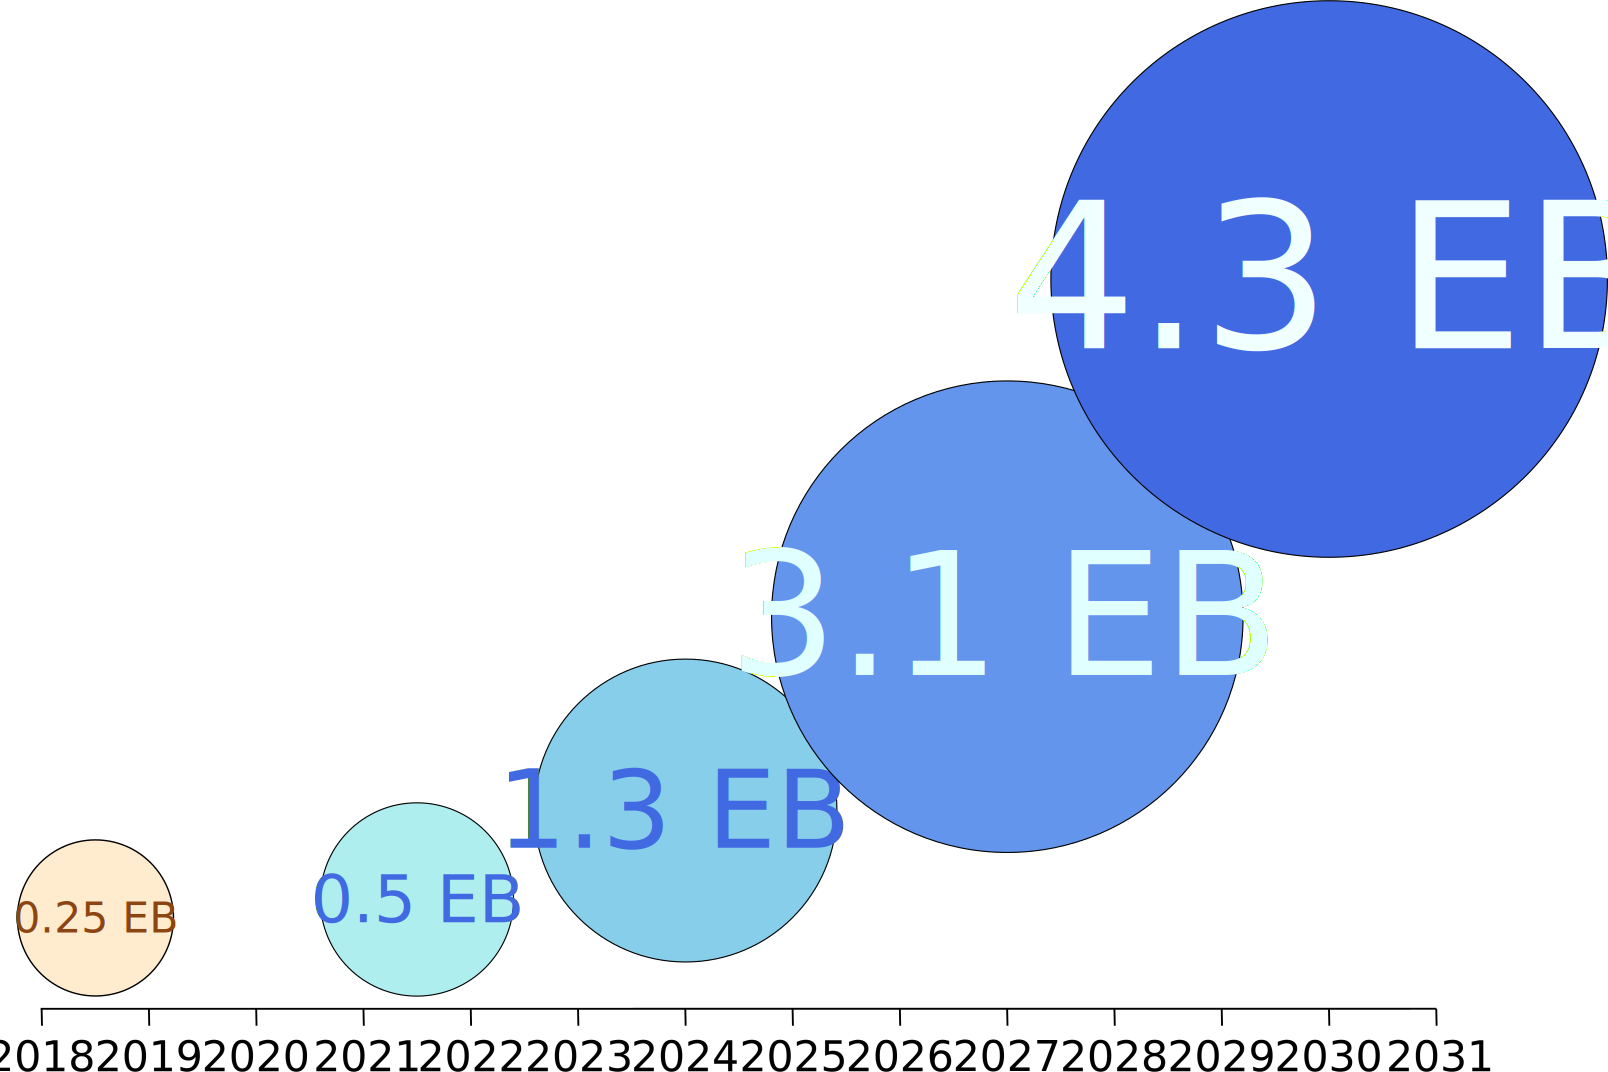
\includegraphics[width=20pc]{images/Storage}\hspace{0.5cm}\vspace{0.25cm}%
   \begin{minipage}[b]{9pc}
      \caption{Predicted Tape Archival Storage Needs for CERN Tier--0 (evolution of total integrated data on tape per year)}
      \label{fig:T0_predicted_storage}
   \end{minipage}
\end{figure}

Increased data rates will also change the way in which archival storage is used. Fig.~\ref{fig:ATLAS_ComputeStorageRequirements}
shows that the anticipated compute and storage needs for the experiments will sharply diverge from the budgets during
LS--3 and Run--4~\cite{atlas_future_chep2018}.
The shortfall in computational resources means that it will no longer be possible to do complete (or comprehensive) data reconstruction,
while the shortfall in disk storage means that it will not be possible to keep all of the data online for
reconstruction and analysis.

\begin{figure}[t]
   \centering
   \includegraphics[width=\textwidth]{images/ATLAS_ComputeStorageRequirements.png}%
   \caption{Predicted Compute and Storage Needs against Flat Budget Model for ATLAS}
   \label{fig:ATLAS_ComputeStorageRequirements}
\end{figure}

In response to these constraints, the LHC experiments are proposing to make much heavier use of tape, as it is a much
more economical form of storage than disk. A recent study~\cite{clipper_tco_2015} shows that disk-based storage
solutions are about six times as costly as tape library-based solutions on a Total Cost of Ownership per TB basis. The
cost savings from increased use of tape will allow the experiments to close the gap between resource needs and the budget.

Increasing the use of tape for I/O-intensive workflows implies a more dynamic interaction between the disk and
tape storage systems. The ATLAS collaboration has begun to study the feasability of a ``data carousel'' arrangement~\cite{xin_zhao_tape_usage},
where raw data will be stored offline on tape and staged back to disk in discrete chunks for online reconstruction
and analysis.

CTA is the IT Storage Group's solution to maximise the efficiency of the tape resources to meet these challenges.
It is planned that data from the LHC experiments will be migrated from CASTOR to
CTA during LS2 in time for full operations to resume at the beginning of Run--3.

This paper is organised as follows:
Sect.~\ref{CASTOR_to_CTA} describes the evolution of CERN's tape storage system from CASTOR to CTA.
Sect.~\ref{EOS_CTA_and_FTS_Integration} describes the integration of CTA with EOS and the File Transfer Service (FTS).
Sect.~\ref{Testing} details the setup and results of our scale and stress testing.
Sect.~\ref{Deployment_and_Migration} outlines the plans for CTA deployment and migration during LS--2.
We summarise in Sect.~\ref{Conclusions}.

\section{CASTOR to CTA}
\label{CASTOR_to_CTA}

After the startup of the LHC, physics analysis payloads moved from CASTOR to EOS, which provides low-latency
disk-only storage~\cite{CERN_data_chep2016}. CASTOR remained as the tape storage system at CERN, with
tape archival transfers and recalls staged in and out of CASTOR's disk system.

To avoid the overhead of maintaining two disk systems, CASTOR disk is replaced by EOS in the new
system. CTA has inherited the CASTOR tape server~\cite{tapeserver_chep2015}, which has been adapted to use
CTA's new control path and metadata. As the CTA system is no longer bound to CASTOR's internal interfaces,
this created an opportunity to redesign the queueing and scheduling features and the tape catalogue, as described below.

\subsection{Queueing and Object Store}
The control of CTA is based on a queueing system for data movement requests. The queues and requests
are stored as objects in a key-value store. For full-scale deployment, the object store backend is Ceph RADOS.
A simpler filesystem-based implementation is used for unit tests.

The agents of the system---tape servers and front ends---collaboratively update this shared storage.
The update procedure is designed so that a process crash will not cause data corruption or loss.
Several maintenance process instances handle failures, \textit{e.g.} re-queueing the requests
that a tape server was working on before it crashed. These maintenance processes free the tape server process
from the need to communicate with EOS. They also handle repack requests.

\subsection{Tape File Catalogue}
The tape file catalogue stores tape file metadata (the physical location of files on tape) and the list of tapes and tape pools.
This catalogue, based on a database, is directly accessed by all agents and collaboratively updated. Care has been taken to
have a simple table layout, not bound to any specific database implementation, to keep dependencies to
a minimum. Full scale deployment is supported on Oracle. An SQLite-based implementation
is used for unit tests.

\subsection{New Scheduling Features}
The control path layout of CTA allows each tape server to schedule its own activity with a global view of the system.
This includes pre-empting the current tape mount to yield to a higher-priority one. This feature renders resource reservation
unnecessary, and maximises the usage of the tape drives. Background tasks like repacking profit from 
the bandwidth provided by all idle hardware without increasing the latency of servicing user requests.

\subsection{New Tape Server Features}
The CTA tape server handles unavailable disk files more efficiently than CASTOR because it does not unmount
the tape it is writing to when it encounters a disk file problem. The CASTOR tape server unmounts the tape
when it cannot read a file from disk. This is costly in terms of time and also causes tape hardware to prematurely wear out.

We are investigating how to add read order optimisation to LTO drives, to compensate for the lack of Recommended
Access Order (RAO)~\cite{cristina_msc_thesis}, which is only available on enterprise drives.

\section{EOS, CTA and FTS Integration}
\label{EOS_CTA_and_FTS_Integration}

\subsection{EOS/CTA Instances}
As mentioned in Sect.~\ref{CASTOR_to_CTA}, one of the main goals of CTA to is to delegate disk cache
and staging functions to EOS. CTA will add tape storage to a collection of relatively small EOS instances
(``EOS/CTA instances''), which are dedicated to staging files to and from tape. As with CASTOR, each LHC
experiment will have a dedicated EOS disk staging area. These EOS instances will communicate with a central
CTA instance which manages the shared tape resources at CERN.

The ALICE, ATLAS and CMS experiments each have a large disk-only EOS instance which is used to cache
data between the experiment data acquisition system (DAQ), the compute/batch nodes of reconstruction
and analysis, and the the Tier--1 sites of the LHC Grid. The EOS/CTA instance of each experiment will
sit behind the large disk-only EOS instance. Ideally, all data in and out of the EOS/CTA instance will
pass through the large disk-only EOS instance. This allows us to optimise the size of the disk pool for the
EOS/CTA instance. Staging tape files on the EOS/CTA instance and directly transferring them to the Tier--1
sites is therefore discouraged, but the data paths will be tailored to meet the individual needs of each
experiment.

\subsection{Storage Resource Managers (SRM) and the File Transfer Service (FTS)}
The use of tape-enabled Storage Resource Managers (SRM)~\cite{SRM2_2} will be deprecated at CERN and
will therefore not be supported by the EOS/CTA instances. Experiments will be able to use the File Transfer
Service (FTS)~\cite{FTS3} and/or the Grid File Access Library (GFAL2)~\cite{GFAL2} to transfer their files
in and out of their EOS/CTA instance. As the IT Storage Group maintains both FTS and GFAL2, we can tailor
solutions to enable the removal of tape-enabled SRM at CERN Tier--0. For transfers between Tier--0 and
Tier--1s, FTS supports transfers to and from both SRM-less and SRM-enabled endpoints.

\subsection{Data Archiving to Tape}
To illustrate how an experiment can work with their EOS/CTA instance, here is the anticipated sequence of events
to transfer a raw data file from the DAQ of an experiment to tape:
\begin{enumerate}
\item The experiment uses XRootD to copy the raw data file from the DAQ to the large disk-only EOS instance.
\item The experiment issues an FTS request to transfer the file from the large disk-only EOS instance to the
EOS/CTA instance, using an XRootD Third Party Copy (TPC) transfer.
\item The EOS/CTA instance automatically archives the file to tape once the TPC has completed.
\item The EOS/CTA instance immediately deletes its disk replica of the file once the file has been safely
copied to tape. The file entry remains in the namespace of the EOS/CTA instance.
\item The experiment polls the EOS/CTA instance until the file has been safely archived to tape.
\item The experiment deletes the file from the DAQ.
\item The experiment eventually deletes the file from the large disk-only EOS instance. 
\end{enumerate}

\subsection{Data Retrieval from Tape}
The anticipated sequence to retrieve a file from tape to the disk-only EOS instance is as follows:
\begin{enumerate}
\item The experiment issues a request to FTS to bring online and TPC the file from the EOS/CTA instance
to the large EOS disk-only instance.
\item FTS uses the XRootD plugin of GFAL2 to request the EOS/CTA instance to bring online (retrieve)
the file from tape.
\item FTS uses the XRootD plugin of GFAL2 to poll the EOS/CTA instance for the progress of the bring
online operation.
\item Once the bring online has succeeded, FTS automatically initiates an XRootD TPC between the EOS/CTA
instance and the large disk-only EOS instance.
\item The garbage collectors of the EOS/CTA instance eventually delete the disk replica from the
EOS/CTA instance.
\end{enumerate}

\section{Testing}
\label{Testing}

%\textit{This section will describe our scale tests, stress tests and field tests.}
%Contributors: \textbf{Julien}
%Testing status report: Scale tests, stress tests.
%Field test setup and config/monitoring automation. Anything we can include from the data challenge.
%
%The scale and stress tests show that the system can operate under a load much heavier than what we currently see in operation.
%Fig.~\ref{fig:scale_stress_tests} shows that a single CTA instance can handle requests at 100 Hz. CASTOR typically operates at not more than 10 Hz.

The EOS/CTA software has been deployed on various hardware infrastructures during 2018 to validate its
functionality and performance. This validation process confirmed CTA theoretical performance in the field
and slowly shaped future CTA operations.

The successive setups grew along several dimensions: size, hardware variety and software stack complexity.
CTA service deployment tools and performance monitoring evolved along with the specifications of the
underlying hardware platform and CTA software development.

The first deployment setup was aiming for a minimal hardware infrastructure and operation framework. The goal of this
pre-production EOS/CTA instance was to validate CTA's ability to absorb high file archival-retrieval rates. It
consisted of two 1GB/s EOS disk servers, two tape servers, and 20 virtual tape drives, but no physical drives. This was ideal for testing
tape metadata operations, as nothing is faster than archiving and retrieving small files on a virtual tape server~\cite{mhvtl}.
This setup could deliver over 1 kHz of raw 1 KB file transfer performance. CTA was able to archive and retrieve up
to 10 million files at a sustained 100 Hz rate (Fig.~\ref{fig:scale_stress_tests_archive}).

\begin{figure}[t]
   \vspace{-1cm}
   \centering
   \makebox[\textwidth][c]{
   \begin{subfigure}[b]{0.688\textwidth}
      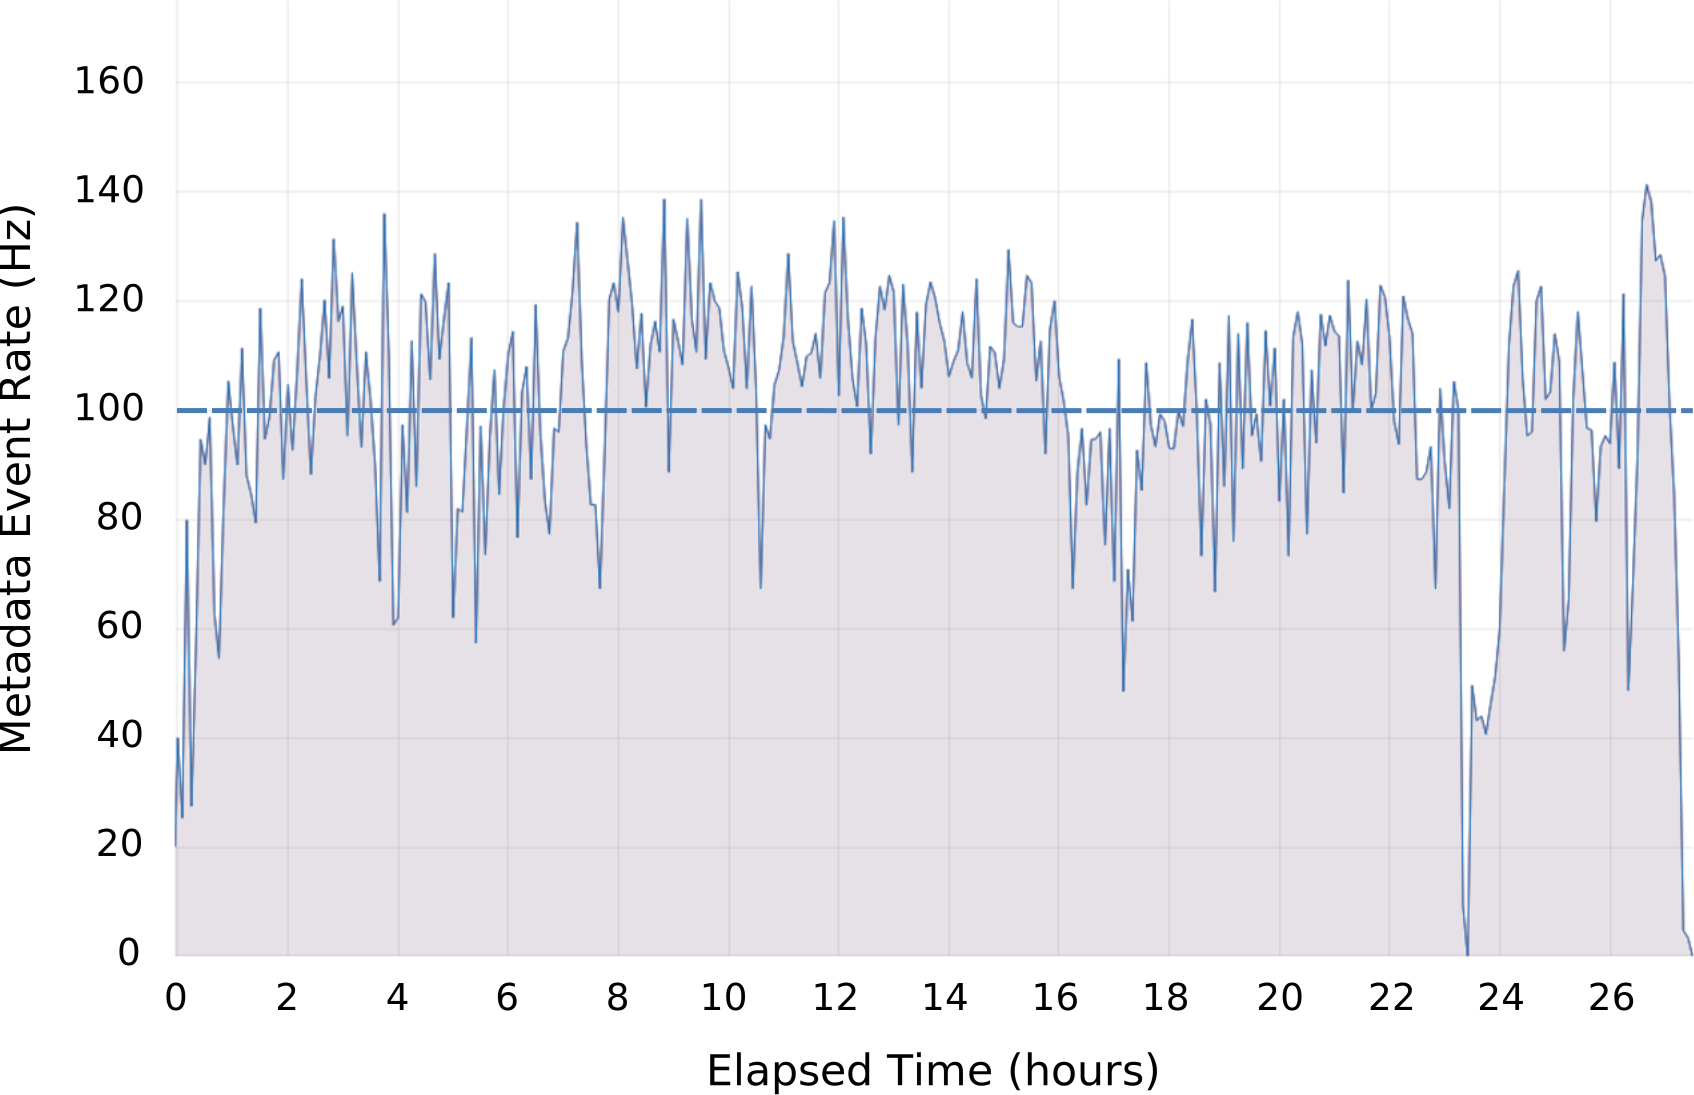
\includegraphics[width=\textwidth]{images/archives_10M}
      \caption{Stage In---10 million files archived in $\approx$27 hours}
      \label{fig:scale_stress_tests_archive}
   \end{subfigure}\hspace{0.5cm}
   \begin{subfigure}[b]{0.312\textwidth}
      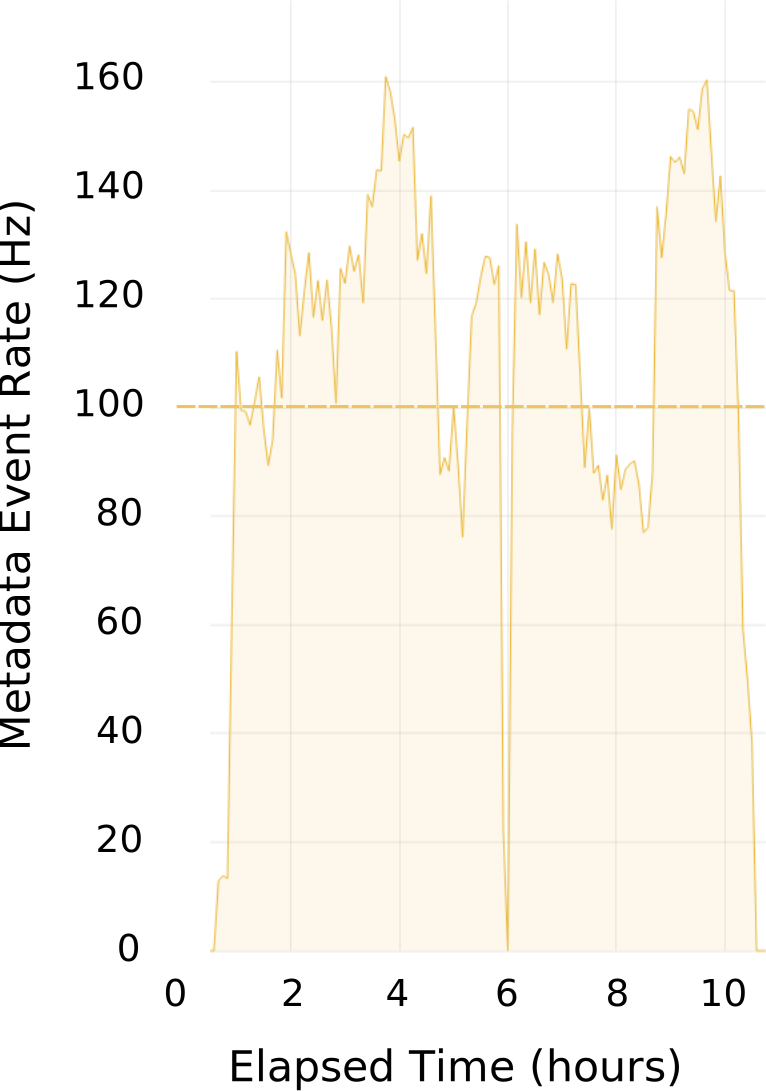
\includegraphics[width=\textwidth]{images/retrieves_4M}
      \caption{Stage Out---4m files in $\approx$10h}
      \label{fig:scale_stress_tests_retrieve}
   \end{subfigure}
   }
   \caption{CTA scale tests and stress tests---performance of metadata operations}
   \label{fig:Deployment}
\end{figure}
\begin{figure}[t]
   \centering
   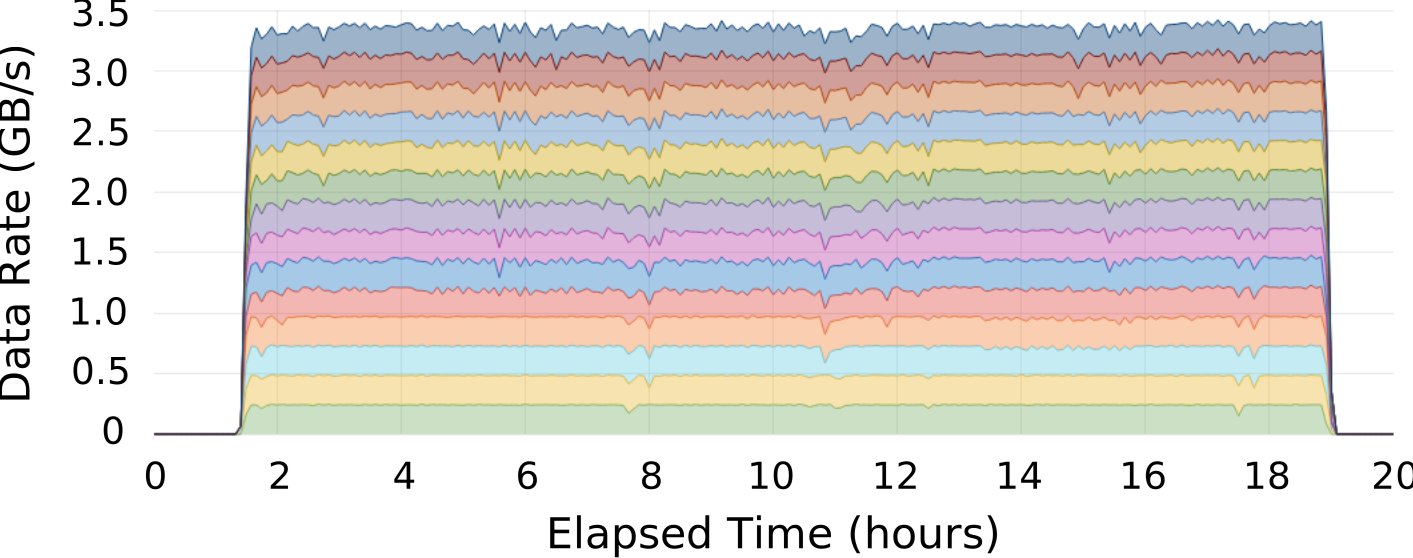
\includegraphics[width=0.8\textwidth]{images/archives_35GB}
   \caption{CTA data transfer rates during the Heavy Ion Data Challenge with 14 tape drives (Sept.~2018)}
   \label{fig:HI_data_challenge}
\end{figure}

The CTA archival metadata rate scales linearly with the number of requests in the queue. The stress tests 
show that CTA can operate under a load one order of magnitude heavier than what we typically see
in CASTOR operations (around 10 Hz). The retrieval stress tests demonstrate
the same scalability properties of CTA software (Fig.~\ref{fig:scale_stress_tests_retrieve}).

After this round of artificially heavy metadata performance validation, EOS/CTA was tested with a more
realistic experiment workflow. The CTA devops team collaborated with the ATLAS Distributed Data Management (DDM)
team to build a significantly more capable testbed: two 10 Gb/s disk servers (raw disk capacity 150 TB),
and four 10TKD tape drives ($\approx1$ GB/s tape archival throughput, see Fig.~\ref{fig:HI_data_challenge}).
This new instance was registered in the ATLAS Grid Information System (AGIS) as a test DDM endpoint and was accessed directly by the ATLAS data transfer tool,
Rucio~\cite{rucio}. Rucio submitted approximately 80k files---200 TB of data---for archival through FTS per test session. The
EOS/CTA instance sustained an average rate of 1.1 GB/s over more than 48 hours and all files were successfully
on tape after 46 hours.

After this initial series of ``real-life'' tests against experiment data flows, CTA throughput performance
was pushed to the limit when CTA participated in the Heavy Ion (HI) Data Challenge.
This consisted of 72 hours of heavy-throughput validation tests with all LHC experiments, to validate CERN IT
Storage infrastructure against LHC Heavy Ion data rates.

%Field Testing:
   %\begin{itemize}
      %\item Goal of user testing is to ensure that all use cases are covered
      %\item Rucio/File Transfer Service (FTS) tests with ATLAS have started
   %\end{itemize}
%Next:
   %\begin{itemize}
      %\item Agree schedule for field testing with all CERN experiments
   %\end{itemize}

\section{Deployment and Migration}
\label{Deployment_and_Migration}

There are currently five instances of CASTOR at CERN, one for each of the main LHC experiments and a Public instance for
everyone else (Fig.~\ref{fig:CASTOR_Deploy}). CASTOR disk is used for staging files to and from tape, while the associated EOS
disk instance is used for reconstruction and analysis (user jobs). When CTA is deployed, each of the CASTOR instances will be replaced
by an EOS/CTA instance (Fig.~\ref{fig:CTA_Deploy}). This ``small'' EOS instance will be optimised for staging files between tape
and disk. Staged files will have a short lifetime, and will be evicted from the staging area as soon as they have been safely
copied to their final destination.

Due to the increased data rates during Run--3, it is desirable to limit the data transfers to\slash from the EOS staging area for data
stored on tape. Therefore it is envisaged that communication path with the experiments and Tier--1s will pass through the large EOS
instance. The small EOS instance will be accessed by privileged experiment accounts and should not be available for user jobs.

\begin{figure}[t]
   \vspace{-1cm}
   \centering
   \makebox[\textwidth][c]{
   \begin{subfigure}[b]{0.525\textwidth}
      \includegraphics[width=\textwidth]{images/CASTOR_Deploy}
      \caption{CASTOR}
      \label{fig:CASTOR_Deploy}
   \end{subfigure}\hspace{0.5cm}
   \begin{subfigure}[b]{0.525\textwidth}
      \includegraphics[width=\textwidth]{images/CTA_Deploy}
      \caption{CTA}
      \label{fig:CTA_Deploy}
   \end{subfigure}
   }
   \caption{Deployment strategies for CASTOR and CTA}
   \label{fig:Deployment}
\end{figure}

\subsection{CTA Deployment}

During the latter part of 2018, we were in communication with each of the four main LHC experiments, to understand
their data management practices and to begin to set up test EOS/CTA instances. The metadata and data transfer tests described in
Sect.~\ref{Testing} established that CTA is performant and reliable under workloads in excess of what we expect to see in production
during Run--3. The main purpose of testing with the experiments is to ensure that the experiment workflows have been properly
understood and to ensure that the experiments' use cases have been covered.

\textbf{ATLAS:} The ATLAS EOS/CTA test instance is in place, comprised of one headnode and three disk servers. Data transfers are
effected using Rucio as the data management system and FTS as the data mover. The workflow maps well to the large EOS instance
for analysis and the small EOS/CTA instance for staging, as ATLAS explicitly do not want a Hierarchical Storage System (HSS);
the experiment wants to remain in full control of where files are stored, on disk or on tape. The IT Storage Group is currently
writing a commissioning document with ATLAS.

\textbf{LHCb:} LHCb's workflow relies on SRM and on staging files directly from CASTOR Tier--0 to the Tier--1s. The IT Storage Group
have worked on integrating GFAL2, FTS and XRootD to avoid the use of SRM, which will be deprecated at CERN. The problem of staging from
CASTOR to grid sites is under discussion with the experiment.

\textbf{CMS:} CMS rely on SRM via PheDex, but PheDex is being deprecated in favour of Rucio, so it is anticipated that the CMS
deployment solution will follow that of ATLAS.

\textbf{ALICE:} Important preliminary work has been done, to move CASTOR operations ``behind'' the large EOS instance, to separate
tape operations from analysis and reconstruction work. Deployment discussions are underway.

\textbf{PUBLIC:} CASTOR Public covers a long tail of small experiments with a broad spectrum of use cases. While the archival needs
of these experiments require only a small fraction of tape resources and operational overhead, a significant amount of analysis
and preparation will have to be done prior to migration. This work will commence once the four main LHC experiment instance
migrations are underway (see Sect.~\ref{Migration_from_CASTOR_to_CTA}).

\subsection{Migration from CASTOR to CTA}
\label{Migration_from_CASTOR_to_CTA}

Once a production instance of EOS/CTA is in place for each experiment, the files will be migrated from CASTOR to CTA.
The format of files on tape is exactly the same in CASTOR and CTA, so no physical movement of data will take place.
Migration is a metadata-only operation; the metadata for each file must be moved from the CASTOR namespace to the CTA
namespace and the EOS namespaces.

The schedule for migration is shown in Fig.~\ref{fig:migration}. Field testing with the experiments began in 3Q2018 and will
continue into 2019. Migration from CASTOR to CTA will take place during the Long Shutdown, when data taking is reduced. The
exact schedule will be planned in discussions with each experiment, to minimise downtime. It will be possible to carry out the
migration in stages, one tape pool (tape family) at a time. CTA will be in full production with all files migrated by the end
of LS--2.

We are investigating the possibility of using an XRootD redirector to further minimise disruption to the experiments. This
would allow CASTOR and CTA to operate in parallel during the migration. Requests would be directed to CASTOR for files which
have not yet been migrated, and to CTA for those which have.

\begin{figure}[t]
   \vspace{-1cm}
   \centering
   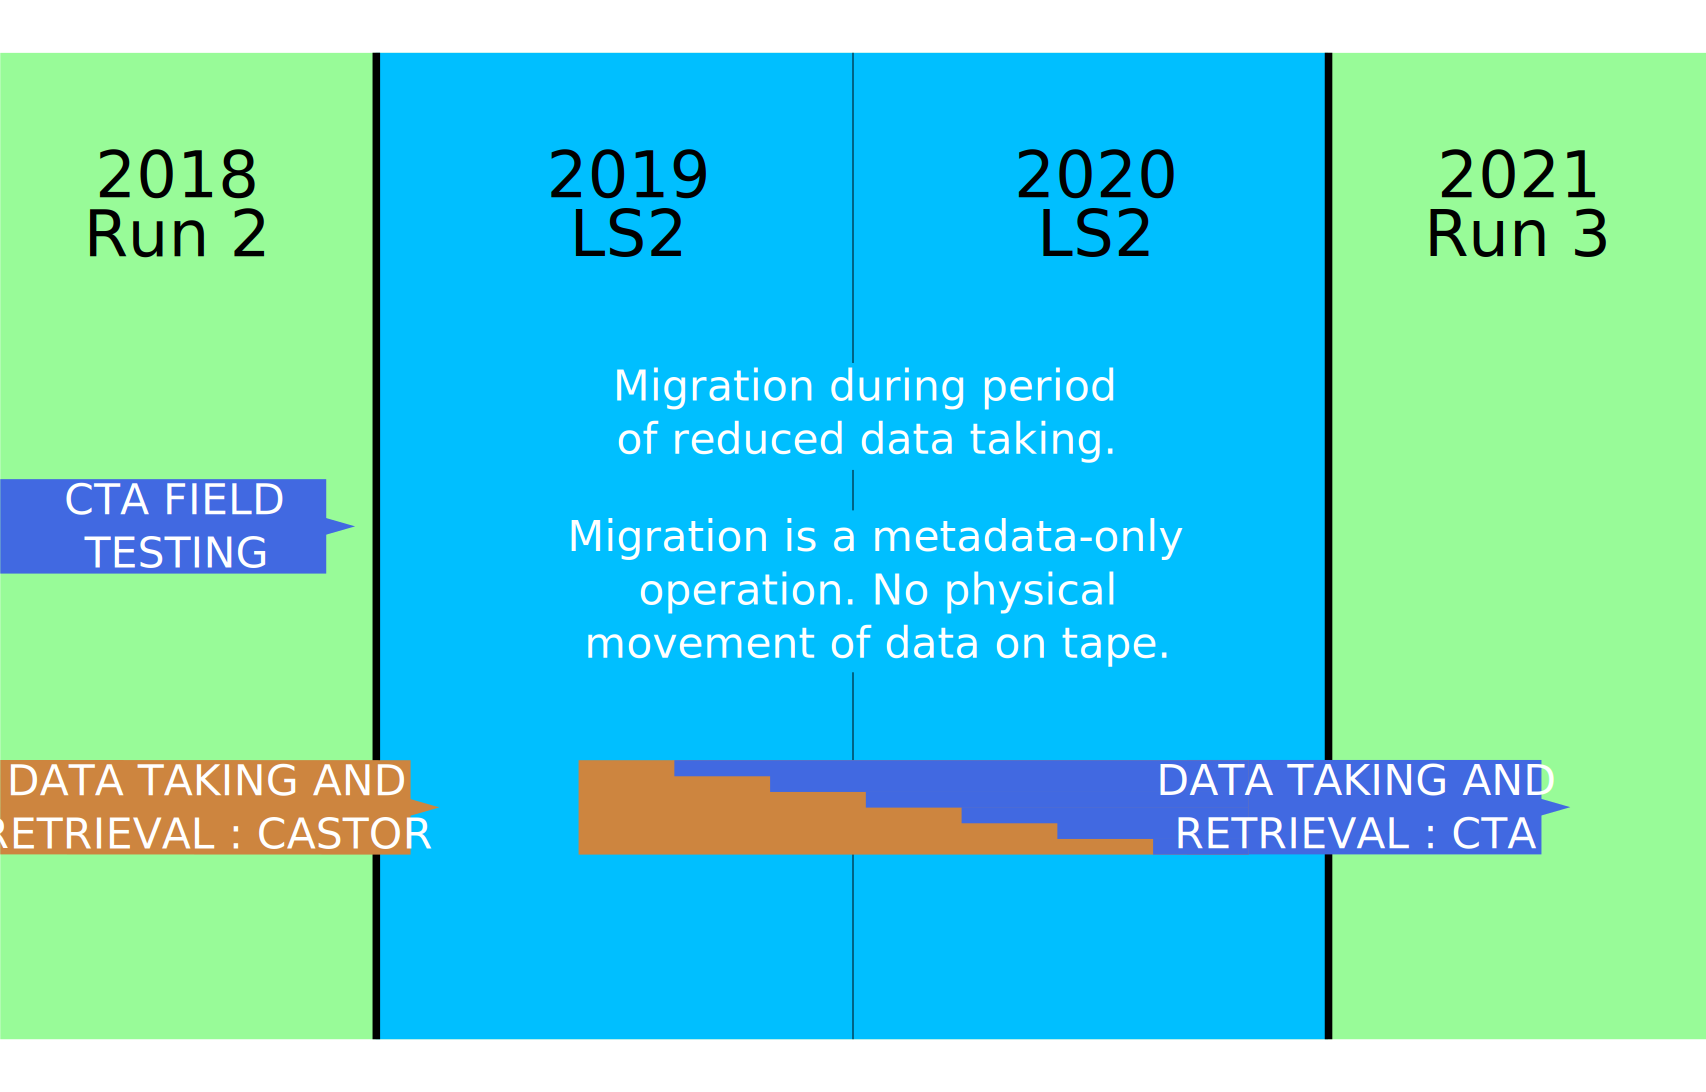
\includegraphics[width=0.8\textwidth]{images/Migration}
   \caption{CASTOR to CTA Migration Schedule}
   \label{fig:migration}
\end{figure}

\section{Conclusions}
\label{Conclusions}

During LS--2, the CERN Tape Archive (CTA) will replace CASTOR as the storage system for the custodial
copy of the physics data at CERN. CTA will address the dual challenges of (a) exponentially increasing
storage needs, and (b) constraints on computing resources available to the experiments, forcing them
to change their workflows to make more use of tape for data reconstruction.

We have described CTA's \textit{raison d'\^etre} as delivering the ``Best of Both Worlds''---EOS disk
and CASTOR tape. The CASTOR tape server has been retained as it is proven to be performant and reliable. 
Using EOS for staging to/from tape avoids the maintenance overhead of two separate disk systems, and
frees the project from the internal interfaces of CASTOR. This allowed a complete redesign of the
queuing and scheduling system, based on a distributed object store, providing a scalable solution for
future archival needs.

During 2018, EOS/CTA was integrated with the File Transfer Service (FTS) and discussions were opened
with the experiments about deployment strategies. The system has been put through its paces with
stringent testing of both metadata and data operations. EOS/CTA test instances for each experiment
are being set up to ensure that the experiments' workflows are understood and handled
properly. Finally, we outlined the strategy for migrating the experiments from CASTOR to CTA during
LS--2, with the goal that CTA will take over as CERN's operational tape archival system for Run--3.

%
% ---- Bibliography ----
%
\bibliography{CHEP2018_CTA}

\end{document}
